% !TEX root=main.tex

\tikzstyle{state}=[shape=circle,draw=blue!50,fill=blue!20]
\tikzstyle{state2}=[shape=circle,draw=purple!50,fill=purple!20]
\tikzstyle{hiddenState}=[shape=circle,draw=gray!50,fill=gray!20,dashed]
\tikzstyle{specialState}=[shape=circle,double=red,draw=blue!50,fill=blue!20,dashed]
\tikzstyle{observation}=[shape=rectangle,draw=orange!50,fill=orange!20]
\tikzstyle{hiddenObservation}=[shape=rectangle,draw=gray!50,fill=gray!20,dashed]
\tikzstyle{lightedge}=[<-,thin]
\tikzstyle{mainstate}=[state,ultra thick]
\tikzstyle{mainedge}=[<-,ultra thick]

\begin{figure*}[!htb]
    \centering
    %\resizebox{0.2\textwidth}{!}{
    \subfloat[{\sc LoopElim} (\S\ref{sec:loop-elim}).]{
    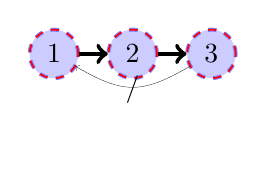
\begin{tikzpicture}[baseline=(s0.base)]
        % states
        \node[specialState] (s0) at (0,0) {$1$};
        \node[specialState] (s1) at (1,0) {$2$}
            edge [<-,ultra thick] (s0);
        \node[specialState] (s2) at (2,0) {$3$}
            edge [<-,ultra thick] (s1);
        %\node[state] (s3) at (3,0) {$4$}
        %    edge [<-,ultra thick] (s2);
        
        %\draw [<-,ultra thin,bend right] (s1) to [looseness=1.25] (s3) node[sloped,draw=none] at (2,-0.45) {$/$};
        \draw [<-,ultra thin,bend right] (s0) to [looseness=1.25] (s2) node[sloped,draw=none] at (1,-0.45) {$/$};

        \node[draw=none] at (0,-1.15)  {};
    \end{tikzpicture}
    %}
    }%
    \qquad    
    %\subfloat[Original prediction with loop (dashed).]{
    \subfloat[{\sc Greedy} (\S\ref{sec:greedy}).]{
    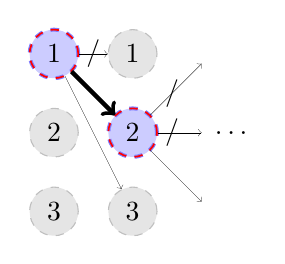
\begin{tikzpicture}[baseline=(s12.base)]
        % first-best
        \node[specialState] (s11) at (0,1)  {$1$};
        \node[hiddenState]  (s12) at (0,0)  {$2$};
        \node[hiddenState]  (s13) at (0,-1) {$3$};

        %\node[hiddenState] (s2) at (1,1.5)  {$2$};
        \node[hiddenState]  (s21) at (1,1)  {$1$};
        \node[specialState] (s22) at (1,0)  {$2$};
        \node[hiddenState]  (s23) at (1,-1) {$3$};
        %\node[hiddenState] (s6) at (1,-1.5)  {$6$};

        \node[draw=none] (s32) at (2,1)  {};
        \node[draw=none] (s31) at (2,0)  {};
        \node[draw=none] (s33) at (2,-1) {};

        \node[draw=none] (s411) at (2.25,0)     {$\ldots$};

        %\draw [->,ultra thin] (s1) to (s2);
        \draw [->,ultra thin]      (s11) to (s21) node [draw=none] at (0.5,1) {$/$};
        \draw [->,ultra thick] (s11) to (s22);
        \draw [->,ultra thin]  (s11) to (s23);
        %\draw [->,ultra thin] (s1) to (s6);

        \draw [->,ultra thin] (s22) to (s32) node [draw=none] at (1.5,0.5) {$/$};
        \draw [->,ultra thin] (s22) to (s31) node [draw=none] at (1.5,0)     {$/$};
        \draw [->,ultra thin] (s22) to (s33);
    \end{tikzpicture}
    }%   
    \qquad
    % \subfloat[Modified prediction with loop removed.]{
    % \begin{tikzpicture}[baseline=(s0.base)]
    %     % states
    %     \node[state] (s0) at (-2,2) {$1$};
    %     \node[state] (s1) at (0,2) {$2$}
    %         edge [<-] (s0);
    %     \node[state] (s2) at (2,2) {$3$}
    %         edge [<-] (s1);
    %     \node[state] (s3) at (4,2) {$4$}
    %         edge [<-] (s2);
    %     \draw [color=white,dashed,bend right] (s1) to [looseness=1.25] (s3);            
    % \end{tikzpicture}
    % }
    %\resizebox{0.2\textwidth}{!}{
    \subfloat[{\sc ILP} (\S\ref{sec:ilp}).]{
    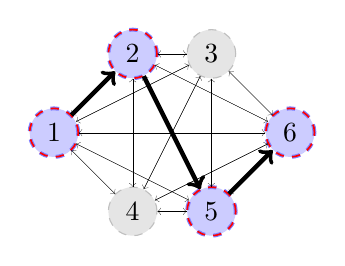
\begin{tikzpicture}[baseline=(s1.base)]
        % first-best
        \node[specialState] (s1) at (0,0)  {$1$};
        \node[specialState] (s2) at (1,1)  {$2$};
        \node[hiddenState]  (s3) at (2,1)  {$3$};
        \node[hiddenState]  (s4) at (1,-1) {$4$};
        \node[specialState] (s5) at (2,-1) {$5$};
        \node[specialState] (s6) at (3,0)  {$6$};

        %\node[draw=none] (juka) at (0,-1.5)  {};

        \draw [->,ultra thick] (s1) to (s2);
        \draw [->,ultra thin] (s1) to (s3);
        \draw [->,ultra thin] (s1) to (s4);
        \draw [->,ultra thin] (s1) to (s5);
        \draw [->,ultra thin] (s1) to (s6);    

        \draw [->,ultra thin] (s2) to (s1);
        \draw [->,ultra thin] (s2) to (s3);
        \draw [->,ultra thin] (s2) to (s4);
        \draw [->,ultra thick] (s2) to (s5);
        \draw [->,ultra thin] (s2) to (s6);    

        \draw [->,ultra thin] (s3) to (s1);
        \draw [->,ultra thin] (s3) to (s2);
        \draw [->,ultra thin] (s3) to (s4);
        \draw [->,ultra thin] (s3) to (s5);
        \draw [->,ultra thin] (s3) to (s6);    

        \draw [->,ultra thin] (s4) to (s2);
        \draw [->,ultra thin] (s4) to (s3);
        \draw [->,ultra thin] (s4) to (s1);
        \draw [->,ultra thin] (s4) to (s5);
        \draw [->,ultra thin] (s4) to (s6);    

        \draw [->,ultra thin] (s5) to (s2);
        \draw [->,ultra thin] (s5) to (s3);
        \draw [->,ultra thin] (s5) to (s4);
        \draw [->,ultra thin] (s5) to (s1);
        \draw [->,ultra thick] (s5) to (s6);    

        \draw [->,ultra thin] (s6) to (s2);
        \draw [->,ultra thin] (s6) to (s3);
        \draw [->,ultra thin] (s6) to (s4);
        \draw [->,ultra thin] (s6) to (s5);
        \draw [->,ultra thin] (s6) to (s1);                    
    \end{tikzpicture}
    %}
    }%
    \qquad
    \subfloat[{\sc List Viterbi} (\S\ref{sec:viterbi}).]{
    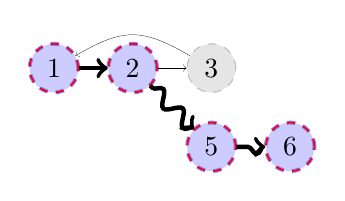
\begin{tikzpicture}[baseline=(s1.base)]
        % first-best
        \node[specialState] (s1) at (0,0)  {$1$};
        \node[specialState] (s2) at (1,0)  {$2$}            
            edge [<-,ultra thick] (s1);

        \node[specialState] (ss1) at (2,-1) {{${5}$}}
        	edge [<-,ultra thick,decorate,decoration={snake}] (s2);
        \node[specialState] (ss2) at (3,-1) {{${6}$}}
            edge [<-,ultra thick,decorate,decoration={snake}] (ss1);

        \node[hiddenState] (s3) at (2,0)  {$3$}            
            edge [<-,ultra thin] (s2);

        % \node[hiddenState] (s4) at (3,0) {$4$}
        %     edge [<-,ultra thin] (s3);

        %\draw [<-,ultra thin,bend left] (s2) to [looseness=1.25] (s4); 
        \draw [<-,ultra thin,bend left] (s1) to [looseness=1.25] (s3); 
    \end{tikzpicture}
    }
    
    %\caption{Example of heuristically removing loops. The nodes are numbered by the POI, with edges denoting order in the sequence. While the modified prediction removes the loop in the original sequence, it is necessarily at the expense of returning a path with fewer number of POIs.}
    \caption{Schematics of different algorithms to return a loop-free prediction.
    Nodes such as
	{\protect\tikz[baseline=(X.base)]{\protect\node[specialState,inner sep=2pt] (X) {\small$1$}}}
    are selected by the algorithm, with thick edges such as
    {\protect\tikz{\protect\coordinate (X) at (0,0) {}; \protect\coordinate (Y) at (0.5,0) {}; \protect\draw[->,ultra thick] (X) to (Y); \protect\node[draw=none] at (0.25,-0.00625) {}}}
    denoting the sequence ordering.
    {\sc LoopElim} removes the loop from the Viterbi solution (here the POI sequence $(1,2,3,1)$), possibly returning a path of shorter length than requested;    
    {\sc Greedy} incrementally selects POIs which have not been selected before, and locally maximises the sub-path score;
    {\sc ILP} solves an integer linear program to find the optimal length $l$ path in a complete graph over POIs;
    {\sc ListViterbi} finds where the second-best sequence diverges from the standard Viterbi sequence ($(1,2,3,1)$ as before); if not loop-free, it finds where the third-best diverges from the second-best, \emph{etc}.
    }
    \label{fig:schematics}
    \vspace{-0.5\baselineskip}
\end{figure*}

